\documentclass{article}

\usepackage[english]{babel}
\usepackage{blindtext}
\usepackage{microtype}
\usepackage{graphicx}
\usepackage{wrapfig}
\usepackage{enumitem}
\usepackage{fancyhdr}
\usepackage{amsmath}
\usepackage{index}
\usepackage{hyperref}
\usepackage[margin=1.0in]{geometry}

\begin{document}
\title{Summary: Control of Body Temperature and Water Balance}
\author{Dowland Aiello}
\date{April 1, 2020}

\maketitle
\tableofcontents
\fancyhf{}

\newpage

\section{Mechanisms for maintaining homeostasis in climatically volatile conditions}

There exist various permutations, or implementations, if you will, of the
general principle of \emph{thermoregulation}---the mechanism through which an
internal temperature can be restricted to an acceptable range conducive to the
survival of a host. Two of these ``implementations'' may be described as
such\footnote{It is not uncommon for an animal to utilize both endothermic and
ectothermic heat regulation mechanisms. Take, for example, the
\href{https://en.wikipedia.org/wiki/Gentoo_penguin}{Pygoscelis papua}---a
member of the Penguin family---. While these birds do regulate body temperature
in a largely endothermic manner, they do warm themselves in the sun. This is an
example of both endothermic and ectothermic behavior. The same is true for the
ectothermic lizard.}:

\begin{itemize}
	\item \textbf{Endothermic heat regulation}: Body heat is derived from the metabolic systems already posessed by a host.
	\item \textbf{Ectothermic heat regulation}: Body heat is derived from an external source.
\end{itemize}

\subsection{Methods of heat exchange}

As does thermoregulation, the act of \emph{heat exchange} can occur in one of
several ways:

\begin{itemize}
	\item \textbf{Conduction}: the transfer of heat between objects that are in
		direct contact with each other.
	\item \textbf{Radiation}: the emission of electromagnetic waves, which can
		transfer heat between objects that are not in direct contact.
	\item \textbf{Convection}: the trnasfer of heat by the movement of air or
		liquid over a surface.
	\item \textbf{Evaporation}: the vaporization of molecules from the surface of a liquid.
\end{itemize}

\subsection{A demonstration of heat exchange}

Each of these disambiguations rely on the principle that heat flows from
an object of higher temperature to one of lower temperature. Yet, they
each serve unique purposes. For example, suppose an ecothermic lizard houses
itself atop a warm rock. The aforementioned modes of heat exchange operate on
the body temperature of the lizard in four ways:

\begin{enumerate}
	\item \emph{Conductively} --- Heat is transfered between the surface of the
		rock and the scales of the lizard through the immediate contact
		established between the rock and the lizard.
	\item \emph{In a radiative manner} --- Energy from the sun warms the
		lizard's back. Furthermore, heat is released from the lizard itself,
		in much the same manner, into the environment.
	\item \emph{In a convectional manner} --- A breeze lifts heat from the
		lizard's tail.
	\item \emph{In an evaporative manner} --- Moisture evaporates from the
		nostrils of the lizard.
\end{enumerate}

\begin{figure}[ht]
	\centering
	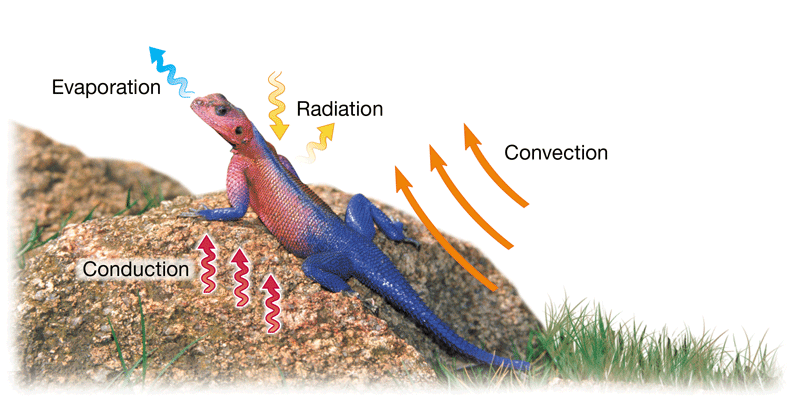
\includegraphics[width=6cm]{lizard_example.png}
	\caption{The lizard from our example}
\end{figure}

\pagebreak

\section{Classifications of thermoregulation adaptations}

While the aformentioned principle of temperature regulation, or
\emph{thermoregulation} can be grouped into two disambiguations: endothermism
and ectothermism, five common implementations of thermoregulation can be
derived from these larger categorizations. More specifically, the 
aforementioned five distinct categorizations are as such:

\begin{enumerate}
	\item \textbf{Metabolic heat production}
	\item \textbf{Insulation}
	\item \textbf{Circulatory adaptations}
	\item \textbf{Evaporative cooling}
	\item \textbf{Behavioral responses}
\end{enumerate}

\end{document}
